\subsection{Environnement de travail}
\begin{frame}\frametitle{Environnement de travail}
\begin{minipage}[c]{.46\linewidth}
	\begin{beamerboxesrounded}[shadow=true,center]{Gestionnaire de version}
		\centering
		
\includegraphics[width=.4\linewidth]{../image/gitLogo.png}
		
\includegraphics[width=.3\linewidth]{../image/githubLogo.png}
	\end{beamerboxesrounded}
\end{minipage}
\hfill
\begin{minipage}[c]{.46\linewidth}
\begin{beamerboxesrounded}[shadow=true]{Gestion de projet}
	\centering
	
\includegraphics[width=.7\linewidth]{../image/lighthouseLogo.png}
\end{beamerboxesrounded}
\end{minipage}
\vfill
\hfil
\begin{minipage}[c]{.6\linewidth}
\begin{beamerboxesrounded}[shadow=true]{Environnement de développement}
	\centering
	
\includegraphics[width=.4\linewidth]{../image/intellijLogo.png}
\end{beamerboxesrounded}
\end{minipage}
\end{frame}
%------------------------------------------------------------------------------
\begin{frame}\frametitle{Méthodologie agile}
\vfill
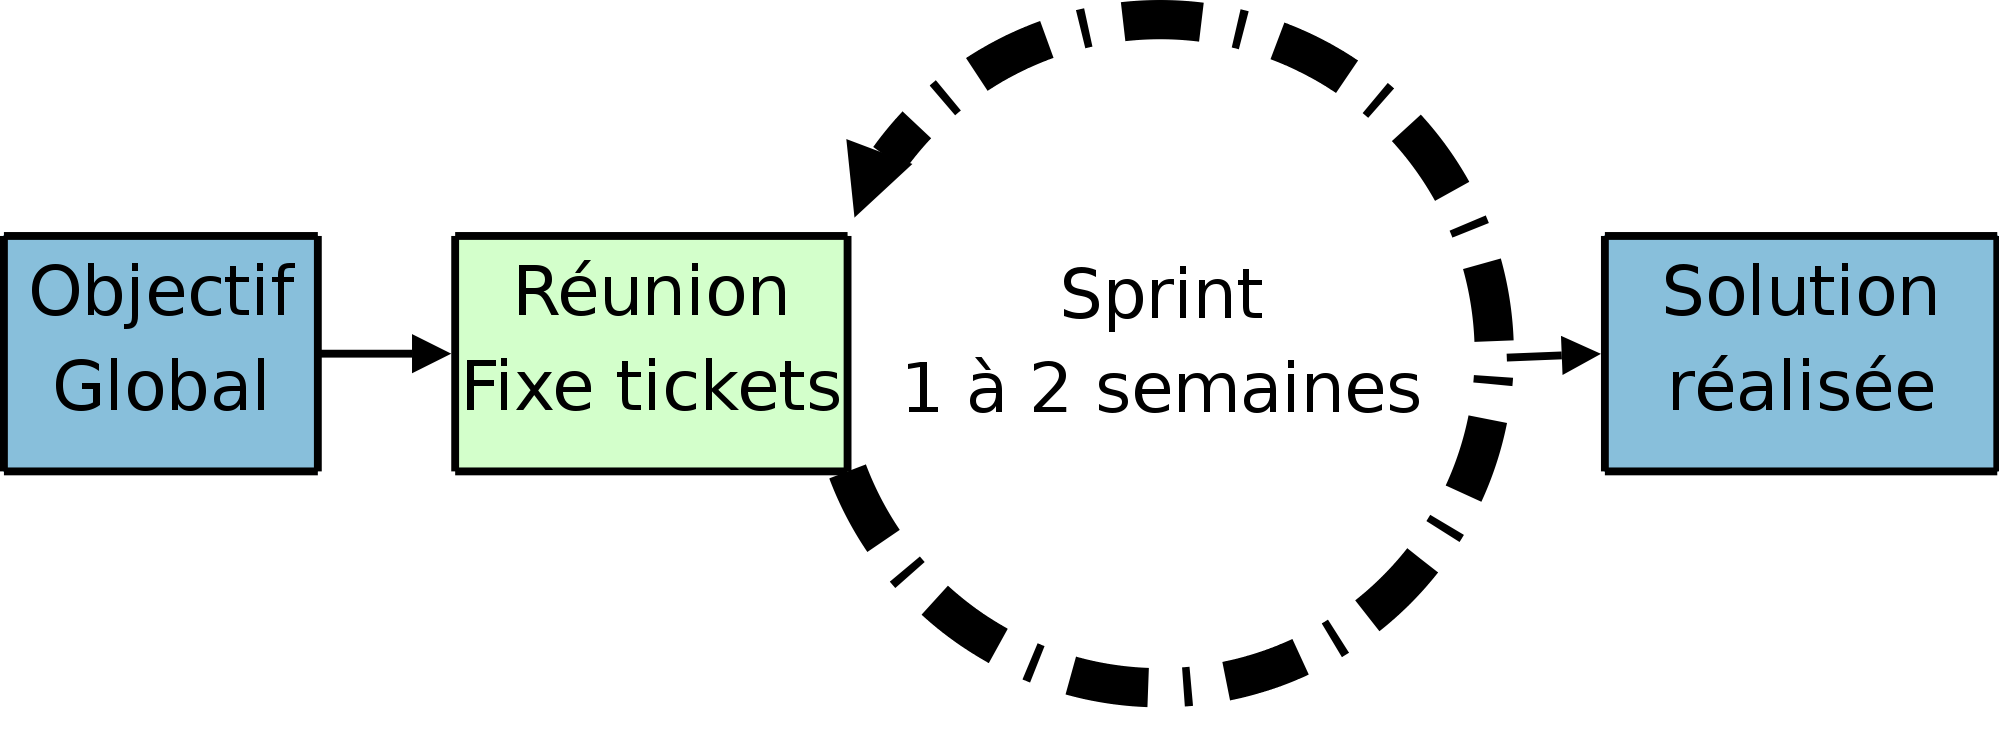
\includegraphics[width=1\linewidth]{../image/agileDev.png}
\end{frame}
%------------------------------------------------------------------------------
\subsection{Transition}
% premier jet, A REVOIR !
\begin{frame}\frametitle{Patron de conception adaptateur}
\begin{minipage}[c]{.46\linewidth}
\begin{beamerboxesrounded}[shadow=true]{Avant}
	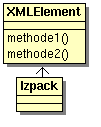
\includegraphics[width=.9\linewidth]{../image/sol_casInitial.png}
\end{beamerboxesrounded}
\end{minipage}
\hfill
\begin{minipage}[c]{.46\linewidth}
\begin{beamerboxesrounded}[shadow=true]{Après}
	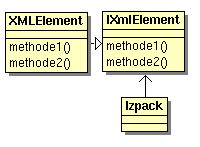
\includegraphics[width=.9\linewidth]{../image/sol_extractionInterface.png}
\end{beamerboxesrounded}
\end{minipage}
\end{frame}
%------------------------------------------------------------------------------
\subsection{Tests}
\begin{frame}\frametitle{Tests unitaires et fonctionnels}
\begin{minipage}[c]{.9\linewidth}
\begin{beamerboxesrounded}[shadow=true]{Tests unitaires}
\begin{itemize}
	\item Assurent un comportement identique\\
	~\\
	\item Testent de nombreux cas\\
	~\\
	\item Couvrent toutes les méthodes\\
\end{itemize}
\end{beamerboxesrounded}
\end{minipage}
\vfill
\begin{minipage}[c]{.9\linewidth}
\begin{beamerboxesrounded}[shadow=true]{Tests fonctionnels}
\begin{itemize}
	\item IzPack\\
	~\\
	\item Glassfish
\end{itemize}
\end{beamerboxesrounded}
\end{minipage}
\end{frame}
%------------------------------------------------------------------------------

% pas sûr de l'utilité si seulement 2 items...
\subsection{Principaux problèmes rencontrés}
\begin{frame}\frametitle{Principaux problèmes rencontrés}
\begin{beamerboxesrounded}[shadow=true]{Principaux problèmes rencontrés}
\begin{itemize}
	\item Xinclude\\
	~\\
	\item Numéros de ligne
\end{itemize}
\end{beamerboxesrounded}
\end{frame}
%------------------------------------------------------------------------------
